\chapter{Какие-то алгоритмы}

Ебанько, сегодня мы тебе расскажем про самые популярные алгоритмы обучения с подкреплением. А за популярность нам зарядили гуглом, насколько они часто упоминаются в свободном доступе.

\section{Какие алгоритмы мы выбрали}

В процессе перекопывания всяких говно-библиотек (\cite{samvelyan19smac}, \cite{MARL-ALGORIGHMS}, \cite{Awesome-MARL}) мы выудили из них этих алгоритмов:
\begin{itemize}[label=---]
	% \item Centralized Q Learning - централизованное Q-обучение;
	\item IQL --- это независимое обучение по кью \cite{DBLP:journals/corr/TampuuMKKKAAV15};
	\item VDN --- это декомпозиция V-функций в сети \cite{DBLP:journals/corr/SunehagLGCZJLSL17};
	\item QMIX --- это факторизация монотонной Q-функции \cite{DBLP:journals/corr/abs-1803-11485};
	\item MAVEN --- это когда несколько чуваков используют вариационное исследование \cite{DBLP:journals/corr/abs-1910-07483};
	      % \item CommNET ---- обучение коммуникации нескольких агентов используя обратное распространение ошибки \cite{DBLP:journals/corr/SukhbaatarSF16};
	\item MADDPG --- это алгоритм DDPG \cite{https://doi.org/10.48550/arxiv.1509.02971} с несколькими чуваками \cite{lowe2017multi};
	\item MAPPO --- это удивительно эффективный PPO \cite{DBLP:journals/corr/SchulmanWDRK17} в среде с несколькими чуваками \cite{DBLP:journals/corr/abs-2103-01955};
	\item IPPO --- это обычный PPO для обучения с подкреплением, но только в среде с одним чуваком.
\end{itemize}

\section{IQL}
Это такой алгоритм, понимаешь, он основывается на Deep Q Learning \cite{Mnih2013PlayingAW}, каждый бомжик контролирует свою сеть. Они играют не связанные друг с другом, но видят одну и ту же кутерьму и действия друг друга. Мы выбрали модифицированный блять эмулятор игровой консоли Atari в качестве среды. В примере с игрой в понг мы проверили среды, где нужно было взаимодействовать или же конкурировать. В ситуациях, где нужно было взаимодействовать, бомжики удерживали мячик на поле как можно дольше.

Но вот есть у него и недостатки, на которые нужно обратить внимание, сука. В частности, он не обеспечивает теоретических гарантий достижения эквилибриума \cite{DBLP:journals/corr/abs-2011-00583}.

Там еще есть некоторые особенности, которые нужно учитывать, блядь:
\begin{enumerate}[label={\arabic*)}]
	\item бомжики принимают только дискретные решения;
	\item алгоритм может использоваться для игр, где нужно взаимодействовать или же конкурировать;
	\item он использует off-policy;
	\item бомжики децентрализованы как во время обучения, так и во время тестирования.
\end{enumerate}

В жизни может случиться так, что бомжики децентрализованы, и только такой подход останется единственным, черт побери.
\section{VDN}

VDN \cite{DBLP:journals/corr/SunehagLGCZJLSL17} пытаются обучить совместную Q--функцию:

\begin{equation}
	Q_{tot} (s, a) = \sum{i \in \mathcal{N}} Q_i(s^i, u^i; \; \theta^i).
\end{equation}
Она, блядь, отличается от IQL тем, что Q-хуйням для каждого хулигана не поступает информация о состоянии и действиях другого хулигана. Таким образом, достигается большая самостоятельность каждого гопника. Метод уступает по всем метрикам методу, описанному ниже, и по этой причине его не берут в сравнениях. Тем не менее, он имеет хватку, чтобы рассматриваться.

Таким образом, можно классифицировать хуету следующими критериями:
\begin{enumerate}[label={\arabic*)}]
	\item Дискретные ходы;
	\item Хуйня для смешанных игр;
	\item Off-policy хуета;
	\item Во время обучения все хулиганы централизованы, а во время тестирования каждый сам за себя.
\end{enumerate}


\section{QMIX}

Слышь, бро, QMIX тоже базируется на VDN, но тут вместо суммы используют факторизацию монотонной Q--функции по ограничению, блять.

\begin{equation}
	\frac{\partial Q_{tot}}{\partial Q_i} \geq 0,\forall i \in \mathcal{N}.
\end{equation}
Чтобы бухнуть условие, QMIX использует 2 дополнительных сети: коктейльную и гипер-хуйню. Авторы босуют эту хуету над VDN на примере кооперативки с матрицей суммы. А вот VQN охуела и не может приколхозить эквилибриума.

Это все ради того, чтобы классифицировать алгоритм по следующим критериям:
\begin{enumerate}[label={\arabic*)}]
	\item дискретные ходы;
	\item алгоритм для мазахистов, которые играют в смешанные игры;
	\item нахуй-policy;
	\item во время учебки агенты в телепузиках, а во время теста нахуй вылетают.
\end{enumerate}

Короче, этот алгоритм улучшает VDN, блять.

\section{MAVEN}

Слушай, чуваки из MAVEN нашли, что эти крысы из QMIX ставят жесткие лимиты, что в свою очередь приводит к тому, что у них тупо говно стратегия и производительность хуже, чем у деда на пивной лавке \cite{DBLP:journals/corr/abs-1910-07483}.

Так вот, эти гопари из MAVEN придумали новый подход, где они связали методы обучения с V-функцией и стратегические методы. Ну и добавили они туда общее латентное пространство, которым управляет иерархическая стратегия.

В общем, они советуют использовать ансамбль генеративных стратегий, чтобы контролировать , и при этом гарантировать монотонность по . И как следствие, получить ровное и последовательное исследование среды.

Ну а на фотке, которую я тебе скинул, видишь архитектуру MAVEN, которая намного круче, чем у тех крыс из QMIX.

\begin{figure}[H]
	\begin{center}
		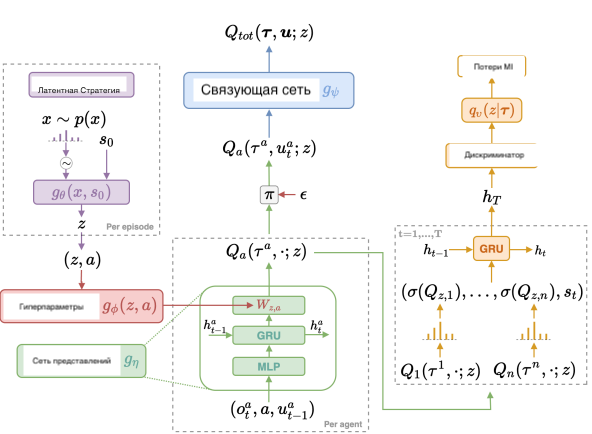
\includegraphics[pages=-, width=140mm]{./inc/img/maven.png}
		\caption{Архитектура MAVEN}
		\label{fig:maven}
	\end{center}
\end{figure}

Ну слышь, бандит, этот алгоритм можно распределить по следующим пунктам:
\begin{enumerate}[label={\arabic*)}]
\item сука, дискретные действия;
\item алгоритм подходит для смешанных игр, понял?
\item блять, off--policy;
\item а во время обучения агенты все центрально, а во время тестирования каждый на своей жопе.
\end{enumerate}

Алгоритм заебистее QMIX и VDN.

% TODO: Таким образом можно классифицировать алгоритм как 1. алгоритм для смешанных игр, 2. агент наблюдает награду за все действия 3. во время обучения агенты централизованны, а во время тестирования децентрализованы;

% \section{CommNet}
% 
% CommNet предлагает ортогональный подход к MARL. Предыдущие алгоритмы не допускают коммуникации агентов.
% В этом подходе, агенты должны придумать способ общения, чтобы достичь цели. Словами являются континуальные вектора.
% 
% \begin{figure}[H]
% 	\begin{center}
% 	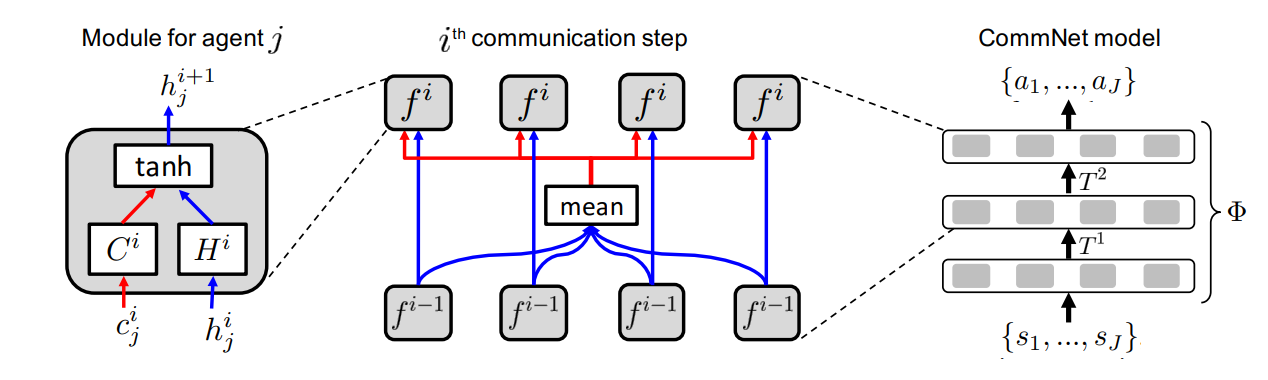
\includegraphics[pages=-, width=140mm]{./inc/img/commnet.png}
% 	\caption{Работа сети CommNet}
% 	\label{fig:commnet}
% \end{center}
% \end{figure}
% 
% Для кодирования состояния используются рекуррентные нейронные сети (\ref{fig:commnet} слева). \( h_j^i \) - скрытое состояние агента \(j\) в момент времени \(i\).
% Нейросеть принимает предыдущее состояние и вектор коммуникации. Вектор коммуникации \(c_j^i\) - это вектор, который агент \(j\) получает от агента \(i\). Вектор коммуникации на следующем шаге - среднее скрытое состояние всех агентов. Вектор коммуникации предоставляется всем агентам на следующем шаге.

\section{Традиционные алгоритмы из обучения с подкреплением}
Эта секция про наши педальные алгоритмы. Вообще, есть один говнокод PPO, который базируется на методе Actor-Critic. Когда несколько агентов в игре, мы используем алгоритм IPPO (независимый PPO), как бы намекая, что нас все ебет и мы сами свои хуи делаем \cite{DBLP:journals/corr/abs-2103-01955}.

Дальше идут алгоритмы, которые делятся на две части: обучение централизованное, а игра децентрализованная (то есть, хулиганы централизованно учились, а теперь разъехались по своим улицам и дерутся). Вот эти чудики называются DDPG и PPO, и у них есть центральная Q-сеть. Есть у них и братаны, MADDPG и MAPPO соответственно, заточенные под игры нескольких агентов \cite{https://doi.org/10.48550/arxiv.1509.02971}. Для полного говнокода мы добавили еще MAA2C - нашу довесочку к A2C, которую мы приготовили специально для наших сука игроков. Также есть IA2C, что в общем-то просто независимая версия A2C, так что особо гонятся за ней не стоит.


Окей, чуваки, сегодня мы на теме IPPO будем ваще угарать. Классификация этого говна может быть сделана по следующим пунктам:
\begin{enumerate}[label={\arabic*)}]
\item смешанные действия;
\item алгоритм для смешанных игр;
\item on--policy;
\item полная децентрализация;
\end{enumerate}

Че, а вы сами в теме, какие сценарии подходят для метода IPPO? Это те, где нет буфера наблюдений среды, агенты сразу в деле обучаются. А еще этот алгоритм зачетный в простоте реализации, и он вообще на полной децентрализации строится.

\subsection*{Вывод}

Мы ёбнули анализ алгоритмов и выбрали самые пиздатые для нашей работы. Давай о них в двух словах, что за звери, как работают и как их можно разобрать на категории.